\chapter{A Tour of the Standard Library}

\section{Types provided by the Standard Library}

\subsection{Strings and Char}

\subsubsection{String type}

String are utilised in the representation of several words combined in a structured manner, i.e. a sentence.
Strings are represented using the double quotation mark around the selection of words 


\begin{lstlisting}[language=C++]
    std::string uninit_example_string;
    std::string example_string = "This is a example string";
\end{lstlisting}

The example above demonstrates both an uninitialized string, i.e. an empty string, and an initialized string.
\\\\
Strings are a type that behave in a similar way to the \textbf{container type} and as such will support all operations that are defined for this type.
The string itself can be regarded as a \textbf{container of bytes that represent the characters that are contained within the sentence}. The string itself can be represented as an \textbf{array of characters} that either has a predetermined size or whose size is determined upon initialization.
The array itself consists of the characters in the order in which they occur in the string itself and is ended with the \textbackslash0 character in the array.

\newpage
\begin{lstlisting}[language=C++]
    using namespace std;

    \\ initialization of the string variable foo with the word 'Hello'

    string foo = "Hello";
    
    \\ Array representation of the same variable as an array of characters that has an undefined length through the use of the square brackets
    
    char foo_array[] = {'H', 'e', 'l', 'l', 'o', '\0'};
\end{lstlisting}

\begin{figure}[h]
    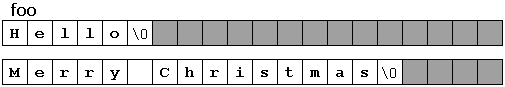
\includegraphics[width=\textwidth]{string_as_array.png}
    \caption{Visual representation of the array nature of the string variable \textit{foo} as it is described in the above code snippet}
\end{figure}

A more in depth discussion of the string and its available methods are discussed in \href{https://cplusplus.com/reference/string/string/}{reference documentation}.

\subsubsection{Char}



